Initially, my intention was to develop the entire software in C++. However, it became evident that a significant amount of time was being wasted on implementing basic functionalities, such as making remote API calls, deserializing JSON objects, or managing simple data in a local SQLite database.

As I have grown accustomed to working with higher-level abstractions that facilitate productivity and enable the maintenance of clean, organized codebases, it became apparent that achieving similar levels of efficiency in C++—a language not primarily designed for such tasks—was considerably more challenging. 

The complexity escalated when I attempted to set up a BLE GATT (Bluetooth Low Energy Generic Attribute) server in C++. I discovered that no high-level abstractions existed for this purpose in any of the available C++ libraries. In contrast, I found an easy-to-use and powerful Python library called \textit{Bless}\footnote{\url{https://pypi.org/project/bless/}}.

This realization led me to a pivotal decision: to shift the networking and data management logic from C++ to Python, thereby leveraging Python's simplicity and robust ecosystem. This move allowed the C++ module to focus on a single, well-defined responsibility: rendering pixels and handling graphics efficiently.

The Python module is designed to serve three primary purposes:
\begin{itemize}
    \item Enable auto-discovery of the matrix for the client application via BLE.
    \item Establish a lightweight LAN COAP server to receive and process commands from the client app.
    \item Manage persistent data, such as user-specified widget configurations using a simple relational SQLite database.
\end{itemize}

\newpage
To facilitate communication between the C++ and Python modules, I implemented a Unix socket, allowing seamless inter-process communication between the two languages.

This is a complete specification of the possible commands that the COAP server can receive:

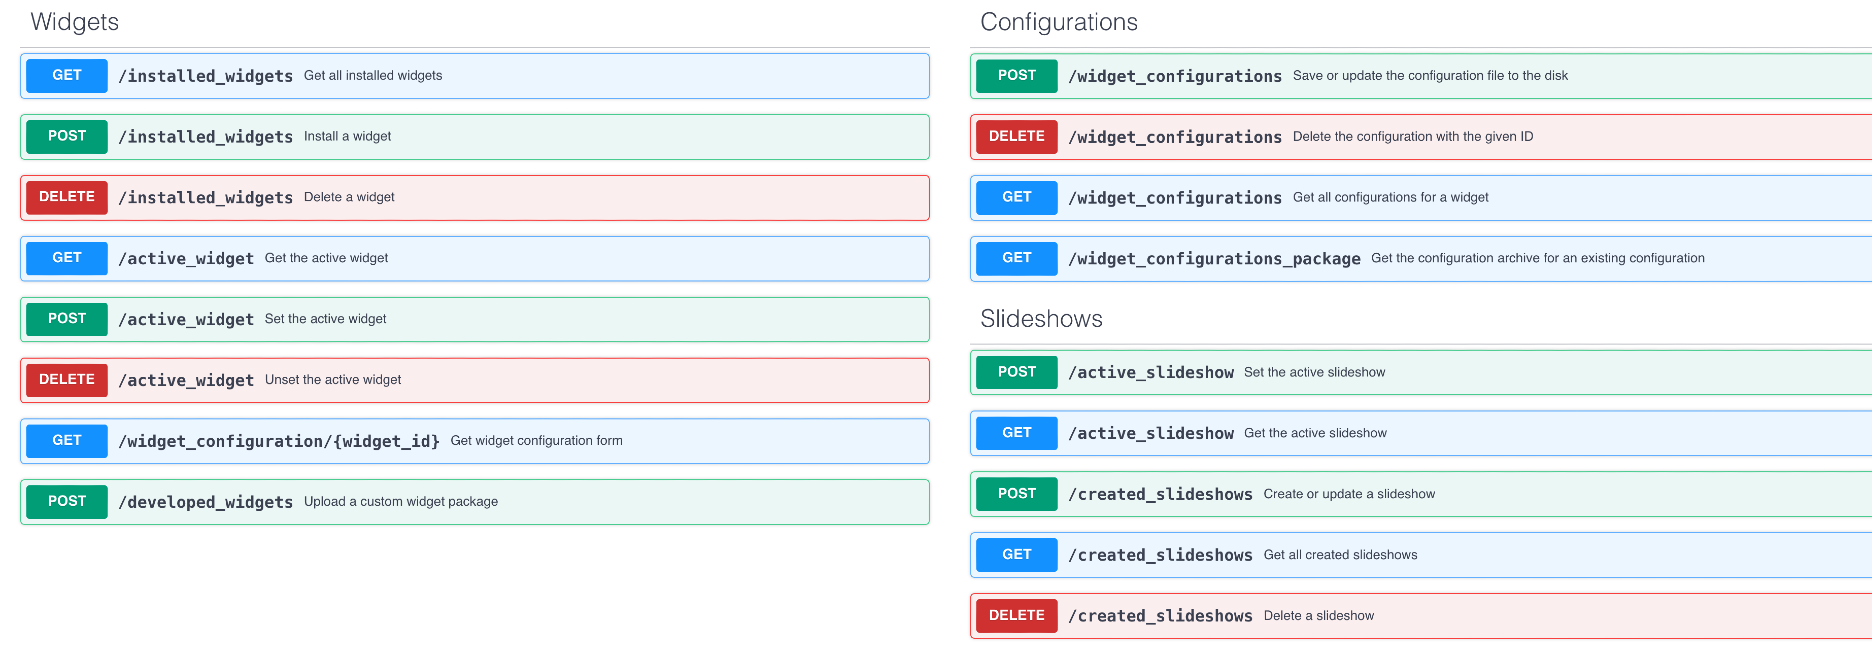
\includegraphics[width=1\textwidth]{tesi/img/coap-swagger.png}

This is an example interaction between the user, the app, the Python module and the C++ module:

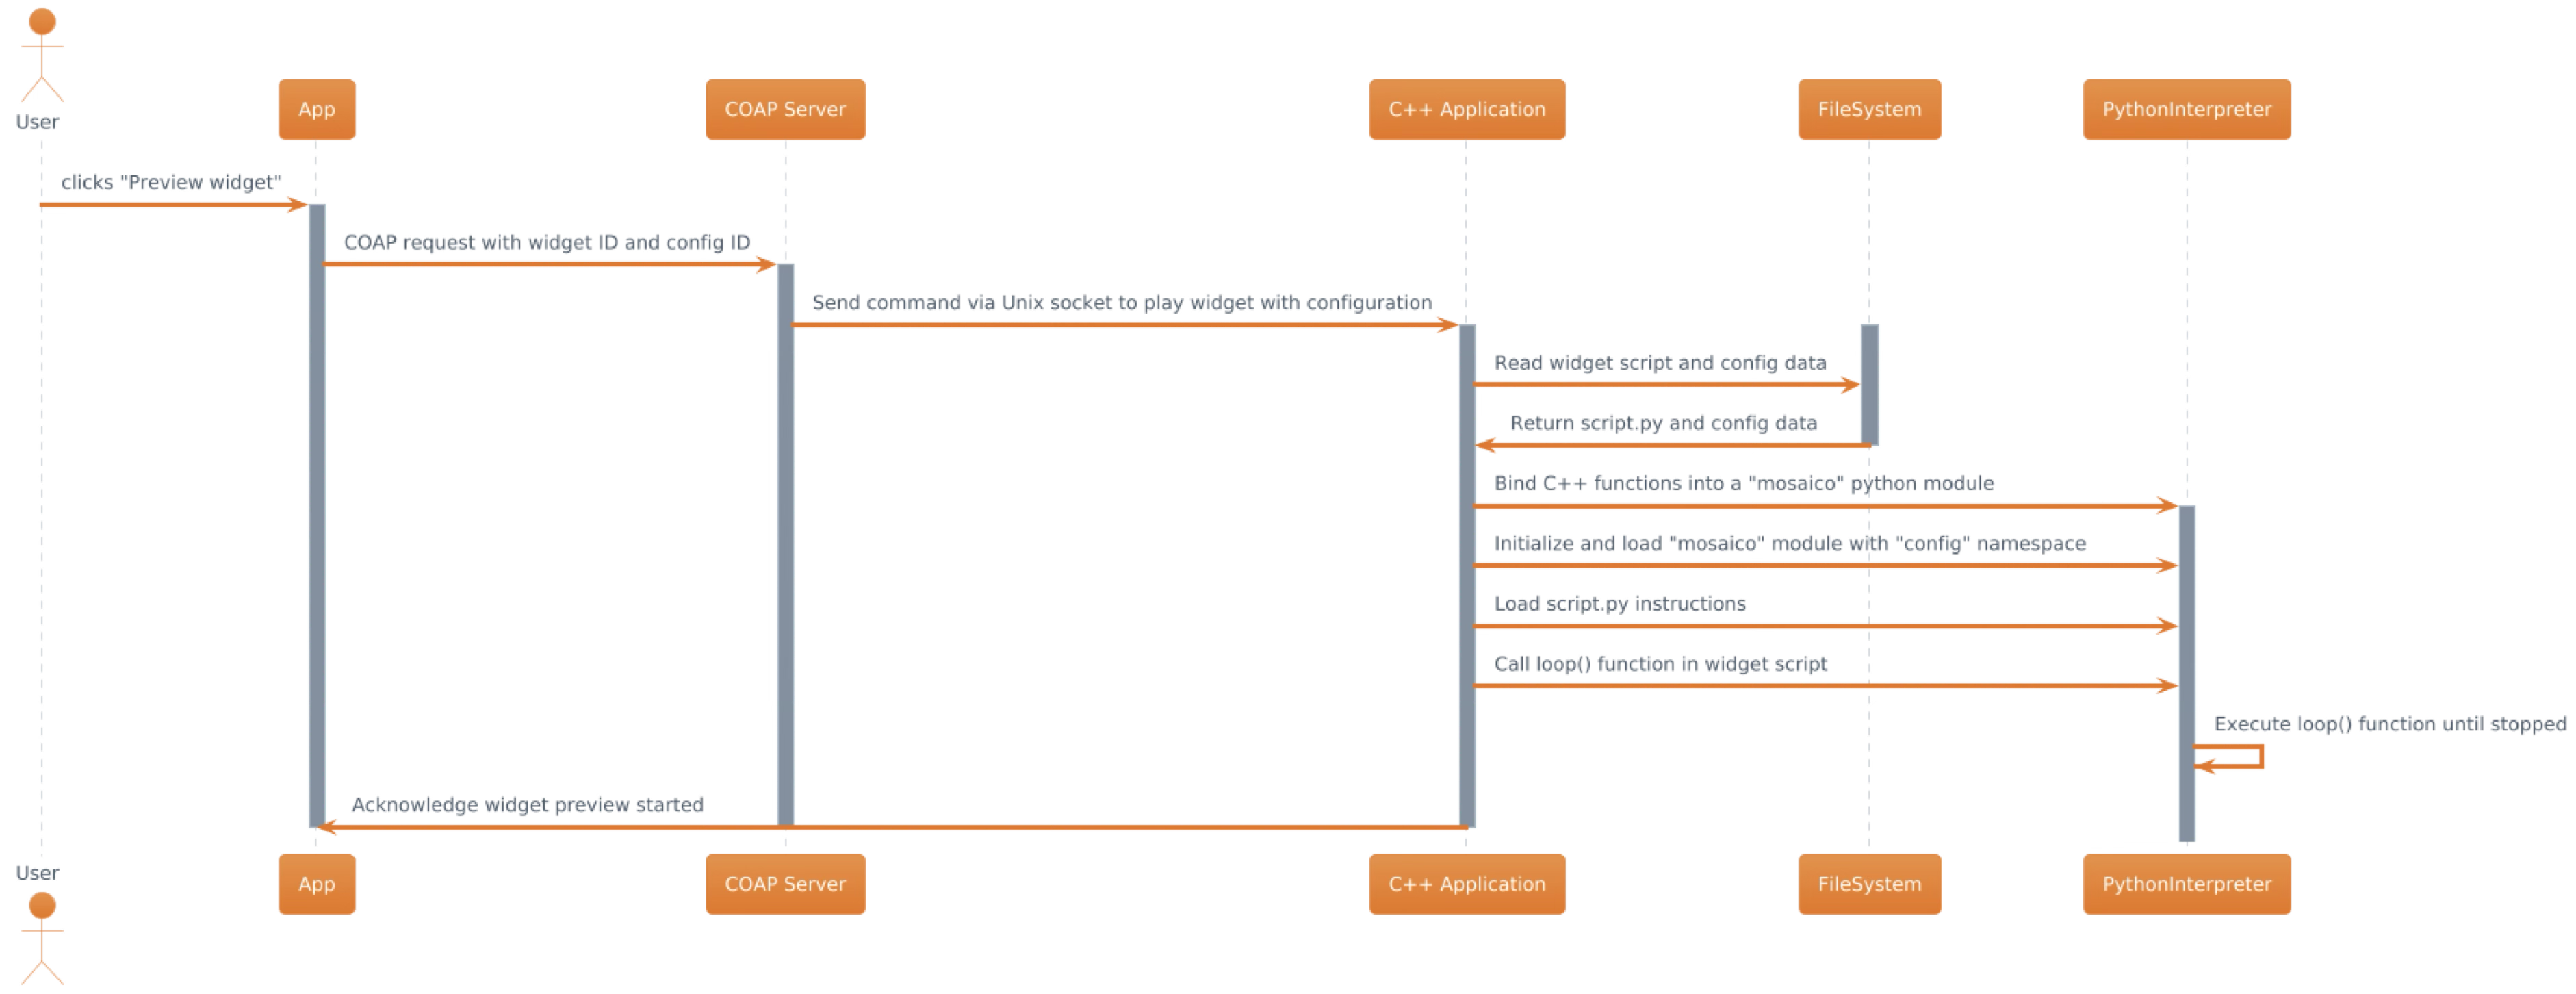
\includegraphics[width=1\textwidth]{tesi/img/activity-install-widget.png}